\appendix
\chapter{Database ER Diagrams}

\section{Entity Relationship Diagram}

This appendix provides visual representations of the database schema relationships.

\subsection{Core Entities}

\begin{figure}[H]
    \centering
    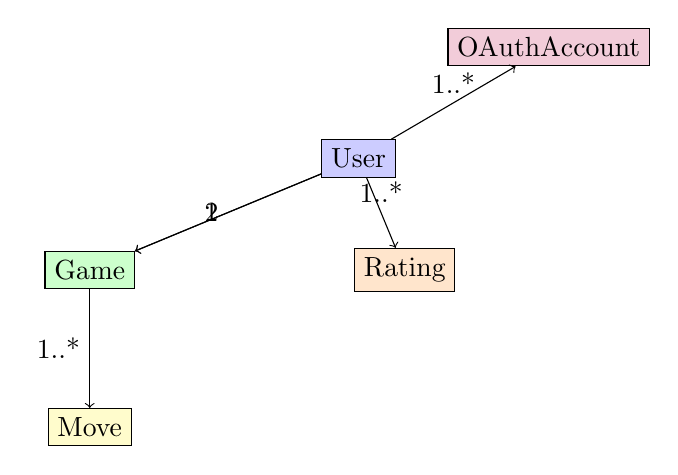
\begin{tikzpicture}[node distance=2cm]
        % User
        \node[rectangle, draw, fill=blue!20] (user) {User};
        
        % Game
        \node[rectangle, draw, fill=green!20, below left of=user, xshift=-2cm] (game) {Game};
        
        % Move
        \node[rectangle, draw, fill=yellow!20, below of=game] (move) {Move};
        
        % Rating
        \node[rectangle, draw, fill=orange!20, right of=game, xshift=2cm] (rating) {Rating};
        
        % OAuth Account
        \node[rectangle, draw, fill=purple!20, above right of=user, xshift=1cm] (oauth) {OAuthAccount};
        
        % Connections
        \draw[->] (user) -- node[left] {1} (game);
        \draw[->] (user) -- node[left] {2} (game);
        \draw[->] (game) -- node[left] {1..*} (move);
        \draw[->] (user) -- node[above] {1..*} (rating);
        \draw[->] (user) -- node[above] {1..*} (oauth);
    \end{tikzpicture}
    \caption{Core Entity Relationships}
    \label{fig:core-entities}
\end{figure}

\subsection{Game-Related Entities}

\begin{figure}[H]
    \centering
    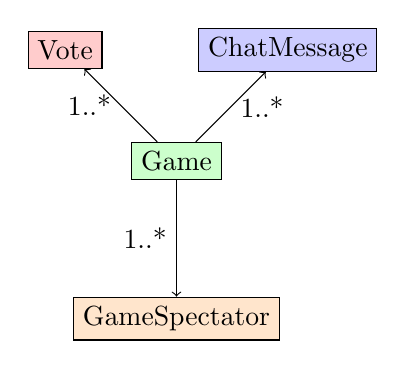
\begin{tikzpicture}[node distance=2cm]
        % Game
        \node[rectangle, draw, fill=green!20] (game) {Game};
        
        % Vote
        \node[rectangle, draw, fill=red!20, above left of=game] (vote) {Vote};
        
        % Chat Message
        \node[rectangle, draw, fill=blue!20, above right of=game] (chat) {ChatMessage};
        
        % Game Spectator
        \node[rectangle, draw, fill=orange!20, below of=game] (spectator) {GameSpectator};
        
        % Connections
        \draw[->] (game) -- node[left] {1..*} (vote);
        \draw[->] (game) -- node[right] {1..*} (chat);
        \draw[->] (game) -- node[left] {1..*} (spectator);
    \end{tikzpicture}
    \caption{Game-Related Entities}
    \label{fig:game-entities}
\end{figure}

\subsection{Academy Entities}

\begin{figure}[H]
    \centering
    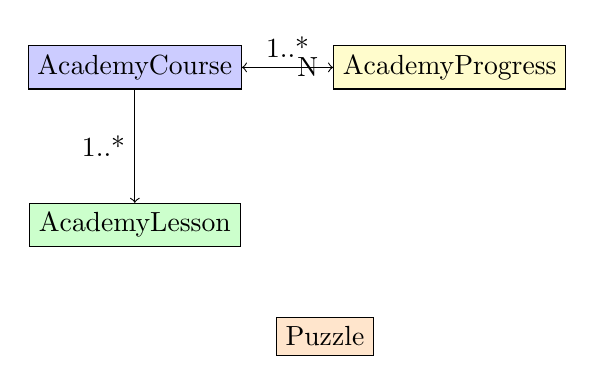
\begin{tikzpicture}[node distance=2cm]
        % Course
        \node[rectangle, draw, fill=blue!20] (course) {AcademyCourse};
        
        % Lesson
        \node[rectangle, draw, fill=green!20, below of=course] (lesson) {AcademyLesson};
        
        % Progress
        \node[rectangle, draw, fill=yellow!20, right of=course, xshift=2cm] (progress) {AcademyProgress};
        
        % Puzzle
        \node[rectangle, draw, fill=orange!20, below right of=lesson, xshift=1cm] (puzzle) {Puzzle};
        
        % Connections
        \draw[->] (course) -- node[left] {1..*} (lesson);
        \draw[->] (course) -- node[above] {1..*} (progress);
        \draw[->] (progress) -- node[right] {N} (course);
    \end{tikzpicture}
    \caption{Academy Entity Relationships}
    \label{fig:academy-entities}
\end{figure}

\subsection{Social Entities}

\begin{figure}[H]
    \centering
    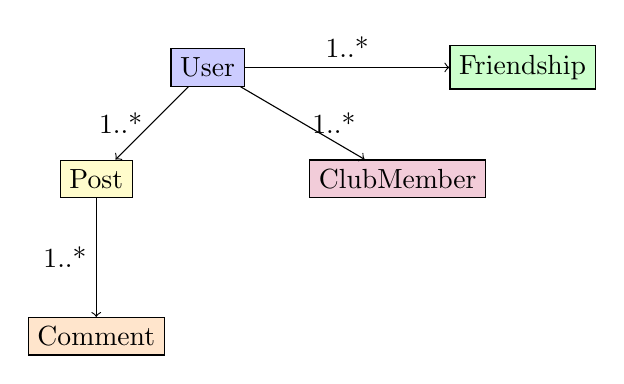
\begin{tikzpicture}[node distance=2cm]
        % User
        \node[rectangle, draw, fill=blue!20] (user) {User};
        
        % Friendship
        \node[rectangle, draw, fill=green!20, right of=user, xshift=2cm] (friendship) {Friendship};
        
        % Post
        \node[rectangle, draw, fill=yellow!20, below left of=user] (post) {Post};
        
        % Comment
        \node[rectangle, draw, fill=orange!20, below of=post] (comment) {Comment};
        
        % Club Member
        \node[rectangle, draw, fill=purple!20, below right of=user, xshift=1cm] (club) {ClubMember};
        
        % Connections
        \draw[->] (user) -- node[above] {1..*} (friendship);
        \draw[->] (user) -- node[left] {1..*} (post);
        \draw[->] (post) -- node[left] {1..*} (comment);
        \draw[->] (user) -- node[right] {1..*} (club);
    \end{tikzpicture}
    \caption{Social Entity Relationships}
    \label{fig:social-entities}
\end{figure}

\subsection{Payment Entities}

\begin{figure}[H]
    \centering
    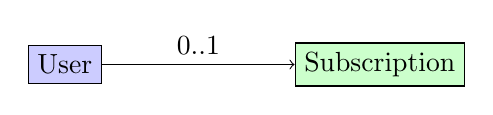
\begin{tikzpicture}[node distance=2cm]
        % User
        \node[rectangle, draw, fill=blue!20] (user) {User};
        
        % Subscription
        \node[rectangle, draw, fill=green!20, right of=user, xshift=2cm] (subscription) {Subscription};
        
        % Connections
        \draw[->] (user) -- node[above] {0..1} (subscription);
    \end{tikzpicture}
    \caption{Payment Entity Relationships}
    \label{fig:payment-entities}
\end{figure}

\section{Table Relationships Summary}

\subsection{One-to-Many Relationships}

\begin{itemize}
    \item User → Games (as white player)
    \item User → Games (as black player)
    \item User → Ratings
    \item User → Votes
    \item User → Chat Messages
    \item User → Posts
    \item User → Comments
    \item Game → Moves
    \item Game → Votes
    \item Game → Chat Messages
    \item Course → Lessons
    \item Course → Progress
\end{itemize}

\subsection{Many-to-Many Relationships}

\begin{itemize}
    \item User ↔ User (Friendships)
    \item User ↔ Course (Progress)
    \item User ↔ Club (Membership)
\end{itemize}

\subsection{One-to-One Relationships}

\begin{itemize}
    \item User ↔ Subscription
    \item User ↔ OAuth Account (per provider)
\end{itemize}
